\documentclass[onecolumn,12pt]{IEEEtran}

\usepackage[left=1in,right=1in,bottom=0.95in,nohead,nofoot]{geometry}
\usepackage{graphicx}

\begin{document}
\title{Informe Laboratorio 2}
\author{Redes de Datos}
%\vspace{3mm}

\begin{figure}[h]

\includegraphics[width=0.50\textwidth]{logo_udp.png}
\label{fig:mesh1}
\\
\\
\\
\\
\\
\maketitle
\end{figure}
\begin{center}
Integrantes:\\
\hfill \\
Gonzalo Felipe\\
Andres Hernandez\\
Franco Centeno\\
\hfill \\
\hfill \\
\hfill \\
\hfill \\
\ \hfill \\
Profesor:\\
Jose Perez\\ \hfill \\
Ayudante:\\
Alexis Inzunza\\
\end{center}

\newpage
\title{Indice}
\author{ }
\maketitle
\hrule
\tableofcontents


\newpage
\section{CONSTRUCCION DE UN CABLE DIRECTO}
\hfill \\

En la primera actividad se tendra que armar un cable directo, para esto se debera tener en cuenta el diagrama entregado de la especificacion T568-A y T568-B.\\
Se pondra a disposicion del equipo un alicate RJ45, un trozo de cable de red, dos rosetas RJ45.\\
El cable directo posee la caracteristica de que en ambos extremos tiene la misma configuracion, aca por ejemplo se escogera la T568-A como se muestra en la figura:

\begin{figure}[h]
\caption{Cable Directo}
\centering 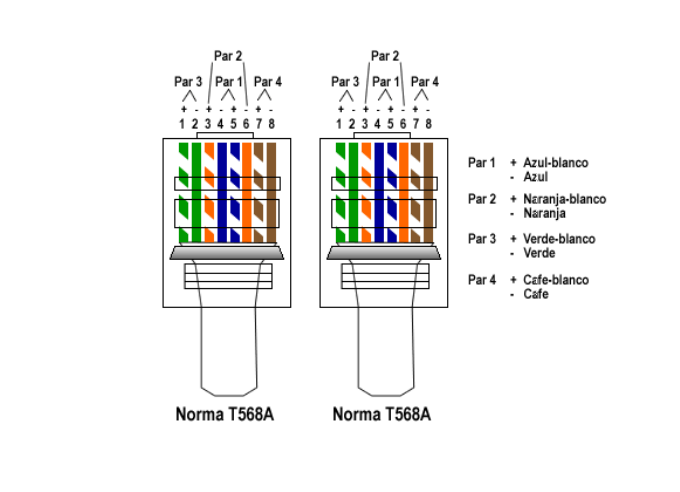
\includegraphics[width=0.75\textwidth]{Directo.png}
\end{figure}




Para armar el cable UTP proseguimos a quitar 5 cm. de la envoltura de ambos extremos del cable, organizamos los pares de acuerdo a la norma T568-A, intentamos mantener las trenzas para inhibir el ruido. Aplanamos y enderezamos los pares y luego cortamos la punta de ellos para que quedaran del mismo largo y rectos. Una vez hecho esto, procedimos a insertar los hilos en el cabezal RJ45, nos aseguramos de que los hilos entraran correctamente.
\\ \hfill

Una vez los cables puestos en el orden correcto dentro del cabezal RJ45, nos aseguramos que todos esten aproximadamente a la misma altura, y luego insertamos el cabezal RJ45 en el alicate para crimpear el extremo, apretandolo firmemente. Finalmente verificamos si el resultado final estaba funcionando correctamente.



\newpage

\section{CONSTRUCCION DE UN CABLE CRUZADO}
\hfill \\

La segunda actividad consiste en armar un cable cruzado, para esto tuvimos que tener en cuentas los diagramas de las dos configuracion, T568-A y T568-B, ya que para hacerlo se necesitara tener cada extremo con una configuracion distinta.
Para construir el cable seguimos las mismas instrucciones que en el cable directo.

\begin{figure}[h]
\caption{Cable cruzado}
\centering 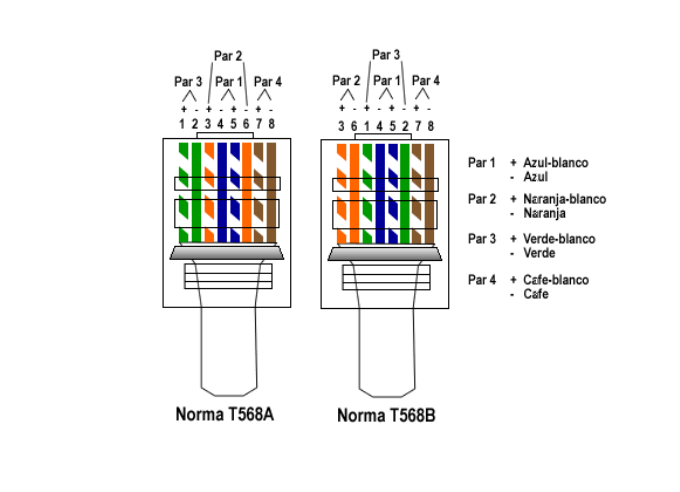
\includegraphics[width=0.75\textwidth]{Cruzado.png}
\caption{Alicate RJ45}
\centering 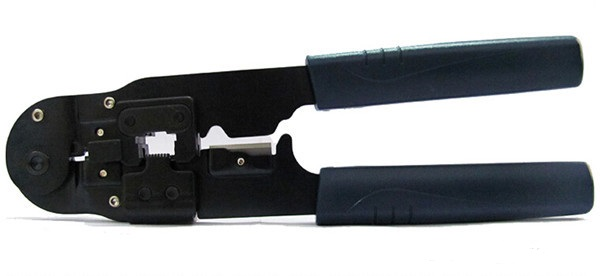
\includegraphics[width=0.75\textwidth]{AlicateRJ45.jpg}
\end{figure}

\newpage
\section{CUESTIONARIO E INVESTIGACION}
\hfill \\

\textbf{1. Describa brevemente las categorias existentes de cable UTP y sus usos.}\\
\hfill \\
\textbf{Cat. 1} Este cable fue disenado para comunicaciones telefonicas \\
\textbf{Cat. 2}	Este tipo de cable de par trenzado no protegido para conexio de antiguos terminales como el IBM 3270.Esta categori de cable es capaz de transmitir datos hasta 4 Mbit/s.
\textbf{Cat. 3}	Es un cable trenzado capaz de trasportar 10 Mbit/s con un posible ancho de banda de 16 MHz
Clase C	10BASE-T and 100BASE-T4 Ethernet	Descrito en la norma \\EIA/TIA-568.\\   
\textbf{Cat. 4}	Es un cable que consiste en 4 cables UTP con una velocidad de datos de 16Mbit/s y un rendimiento de hasta 20 MHz. Fue usado en redes token ring.\\
\textbf{Cat. 5}	Este cable puede transmitir datos a velocidades de hasta 10000 Mbps a frecuencias de hasta 100 MhZ.Estos cables pueden ser blindados o sin blindar. Este tipo de cables se utiliza a menudo en redes de ordenadores como Ethernet, y también se usa para llevar muchas otras señales como servicios básicos de telefonía, token ring, y ATM.\\
\textbf{Cat. 5e} Este cable es una mejora del cable categoria 5, sus aplicaciones son para 100BASE-TX y 1000BASE-T Ethernet.\\
\textbf{Cat. 6}	Este cable es un estadar de cables para Gigabit Ethernet y otros protocolos de redes que es retrocompatible con los estándares de categoría 5/5e y categoría 3. La categori 6 posee caracteriticas y especificaciones para crosstalk y ruido. El estadar de cable es utilizable para 10BASE-T, 100BASE-TX y 1000BASE-TX (Gigabit Ethernet). Alcanza frecuencias de hasta 250MHz en cada par y una velocidad de 1Gbps.\\
\textbf{Cat. 6a} Este cable sirve para transmitir en 10 Gbps sobre par trenzado, con frecuencias y paraetros de transmisio definidos hasta 500 MHz, son definidas por la norma ANSI/TIA-568-C.2. Debido a la alta frecuencia necesaria para soportar esta tasa de transferencia, esta norma incluye un parámetro de transmisio denominado AlienCrosstalk (ANEXT).\\
\textbf{Cat. 7}	600 MHz Clase F		Cable U/FTP (sin blindaje) de 4 pares. \\
\textbf{Cat. 7a}	1000 MHz Clase F	Para servicios de telefonia, Television por cable y Ethernet 1000BASE-T en el mismo cable.	Cable S/FTP (pares blindados, cable blindado trenzado) de 4 pares. \\
\textbf{Cat. 8}	1200 MHz	Norma en desarrollo. Aun sin aplicaciones. \\
\textbf{Cat. 9}	25000 MHz	Norma en creacion por la UE. \\
\textbf{Cat. 10}	75000 MHz	Norma en creacion por la G.E.R.A(RELATIONSHIP BETWEEN COMPANIES ANONYMA G) e IEEE.\\
\hfill \\

\textbf{2. ¿Para que situaciones debería utilizar un cable STP? Explique.}\\
\hfill \\
Es utilizado en las instalaciones de procesos de datos por su capacidad, tambien se utiliza a menudo en redes de ordenadores como Ethernet, 10 Base-T, 100 Base-T, 1000Base-T, y también se usa para llevar otras señales como servicios básicos de telefonía, Token Ring, FDDI, ISDN, ATM, redes de audio como EtherSound y controles de luz DMX,por sus buenas caracteristicas contra las radiaciones electromagneticas, pero el inconveniente es que es un cable robusto, caro y dificil de instalar.

\newpage
\section{IMAGENES DE LOS RESULTADOS}
\begin{figure}[h]
\caption{Cable Directo:}
\centering 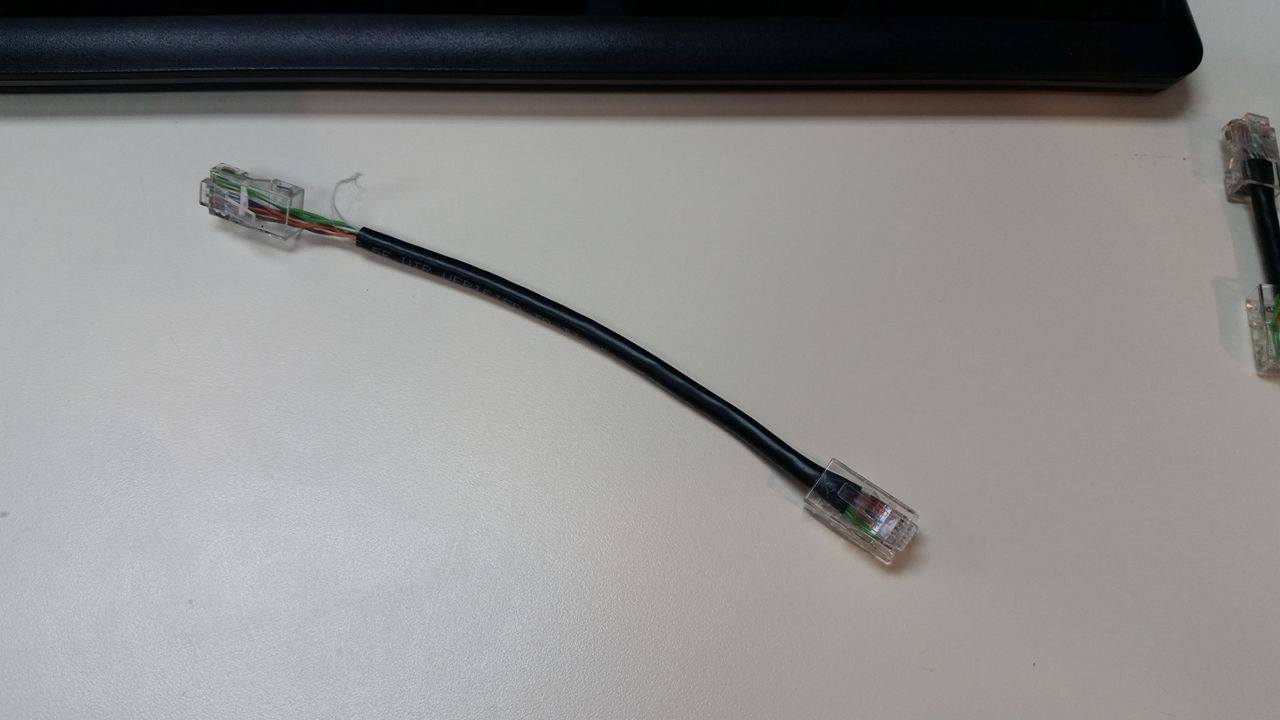
\includegraphics[width=0.75\textwidth]{CableDirecto.jpg}
\end{figure}


\begin{figure}[h]
\caption{Cable Cruzado:}
\centering 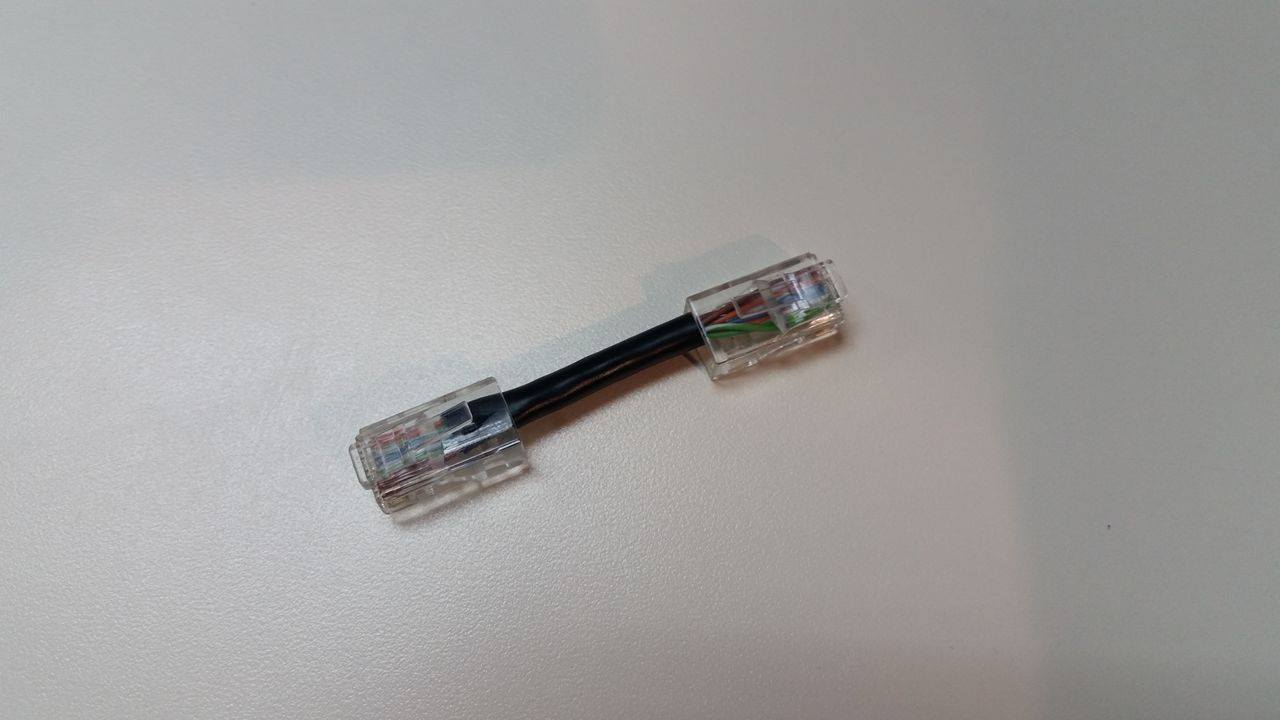
\includegraphics[width=0.75\textwidth]{CableCruzado.jpg}
\end{figure}


\newpage
\section{CONCLUSION}
\hfill \\

El uso de los cable UTP es crucial al momento de hablar de conexiones de tipo red, telefonia o incluso television en algunos casos. Estamos hablando de la union y manejo de informacion, el uso de este tipo de cables, tanto UTP como STP, ha sido indispensables a la hora de montar una red en cualquier parte.
\hfill \\
\hfill \\
\section{BIBLIOGRAFIA}

Categorias cable UTP,
\emph{Wikipedia} \\
\url{https://es.wikipedia.org/wiki/Cable\_de\_par\_trenzado} \\

Categorias cable UTP,
\emph{Slideshare} \\
\url{https://es.slideshare.net/OSWALDODEDE0/tipos-de-cable-utp-12852564} \\

Categorias cable UTP,
\emph{Furukawalatam} \\
\url{http://www.furukawalatam.com/py/productos/?agrupamento=5&categoria=59&nivel1=1&nivel2=2}

\end{document} 
